% $Id: AllegProposal.tex,v 1.8 2000/07/05 21:02:12 culver Exp $
% AllegProposal.tex
% by A. Thall
% 13. Feb 2003
%
% Small edits and a few additions made by R. Roos
% 21 Jan 2007
% Most particularly, the "box" around the thesis statement has been removed,
% section titles have been modified. The section named "Prior work II" has
% been commented out. The \topmargin has been changed to -.5in and the
% change to \parindent has been commented out.
% The filename "nausicaa.eps" has been changed to simply "nausicaa" so that
% pdflatex can be used on the file (and a file named "nausicaa.pdf" has
% been created using the "epstopdf" command).
% Several subsections have been added to illustrate subsection usage.
% The word "comp" has been replaced by "project" or "thesis" throughout.
% Other small changes have been made.
%
% This document provides a sample Senior Project Proposal template for use
% by students in Allegheny's CS and Applied Computing programs.

\NeedsTeXFormat{LaTeX2e}
\documentclass[11pt]{article}

%The following is used by WinEdt to set up cross-referencing to the BibTeX files
%It is NOT commented out---the comment lets it be simply ignored by non-WinEdt LaTeX compilers

%GATHER{mybibtexDB.bib}

\usepackage{setspace}
\usepackage{amsmath}
\usepackage{amssymb}
\usepackage{epsfig}
\usepackage{fancybox}
\usepackage{listings}
\usepackage{algo}
\usepackage{url}
\usepackage{multirow}
\usepackage{tabls}
\usepackage{afterpage}
\usepackage{booktabs}
\usepackage{epsf}
\usepackage{amsmath}   
\usepackage{amsfonts}
\usepackage{amssymb}
\usepackage{amsbsy}
\usepackage{bm}
\usepackage{epsfig}
\usepackage{rotating}
\usepackage{setspace}
\usepackage{tabls}
\usepackage{hhline}
\usepackage{float}

\setlength{\textheight}{9in}
\setlength{\textwidth}{6in}
\setlength{\oddsidemargin}{.25in}
\setlength{\topmargin}{-.5in}  % changed from -.25 by RSR on 1/21/07
%\parindent .5in    % commented out by RSR 1/21/07

%%% MY COMMANDS %%%

\usepackage{graphicx}
\usepackage{tabls}
\usepackage{afterpage}
\usepackage{float}
\usepackage{color}
\usepackage{amsmath,amsthm,amssymb}
\usepackage{verbatim}
\usepackage[parfill]{parskip}
\usepackage{tikz}
\usepackage{subcaption}
\usepackage{soul}
\usepackage[labelfont=bf]{caption}
\usepackage[framemethod=tikz]{mdframed}
\usepackage{multirow}
 
\renewcommand{\thefootnote}{\fnsymbol{footnote}}
\renewcommand{\ss}{\ensuremath{\|s\|}}
\newcommand{\N}{\mathbb{N}}
\newcommand{\Z}{\mathbb{Z}}
\newcommand{\deriv}[2]{\frac{\mathrm{d} #1}{\mathrm{d} #2}}
\newcommand{\pderiv}[2]{\frac{\partial #1}{\partial #2}}
\newcommand{\bx}{\mathbf{X}}
\newcommand{\ba}{\mathbf{A}}
\newcommand{\by}{\mathbf{Y}}
\newcommand{\bj}{\mathbf{J}}
\newcommand{\bs}{\mathbf{s}}
\newcommand{\B}[1]{\ensuremath{\mathbf{#1}}}
\newcommand{\Dt}{\Delta t}
\renewcommand{\d}{\mathrm{d}}
\newcommand{\mom}[1]{\langle #1 \rangle}
\newcommand{\cur}[1]{\left\{ #1 \right\}}
\newcommand{\xl}{{x_{i-1/2}}}
\newcommand{\xr}{{x_{i+1/2}}}
\newcommand{\il}{{i-1/2}}
\newcommand{\ir}{{i+1/2}}
\newcommand{\jl}{{j-1/2}}
\newcommand{\jr}{{j+1/2}}
\newcommand{\FOM}{\ensuremath{\text{FOM}}}

\graphicspath{{figures/}}


%put words in the hyphenation statement if you want to enforce
%how LaTeX should break them (or not) at the end of a line.
%\hyphenation{repre-sen-tations problems exact linear}
\hyphenation{itself}

%%%%%
%% Commented out -- RSR, 1/21/07
%%%%%
% The following provides a box to surround the thesis statement
%\newenvironment{Thesis}%
%{\begin{Sbox}\begin{minipage}{.95\linewidth}}%
%{\end{minipage}\end{Sbox}\begin{center}\fbox{\TheSbox}\end{center}}

\title{A High-Order Low-Order Algorithm with Exponentially-Convergent Monte Carlo for Thermal Radiative Transfer}
\author{Dissertation Proposal \\ Simon Bolding, Nuclear Engineering Department}

\begin{document}


\singlespace
\maketitle

\doublespace
% This sets section-numbering to only include Section and Subsection numbers
\setcounter{secnumdepth}{2}


\section{Introduction}

The ability to accurately model the difficult physics involved in thermal radiative transfer (TRT) is important in high-energy, high-density physics regime.  Applications include inertial confinement fusion and astrophysics applications.  This research will focus on frequency-integrated (grey), one spatial dimension radiative transfer problems. 
The governing equations are the 
radiation and
material energy balance equations, i.e.,\vspace{-0.05in}
\begin{align}\label{ho_cont}
    \frac{1}{c}\pderiv{I(x,\mu,t)}{t} + \mu \pderiv{I(x,\mu,t)}{x} + \sigma_t
    I(x,\mu,t)
&= \frac{\sigma_s}{2} \phi(x,t) +\frac{1}{2} \sigma_a a c T^4(x,t)
    \\ \label{t_cont}
  \rho c_v \pderiv{T(x,t)}{t} &=  \sigma_a \phi(x,t) - \sigma_a a c T^4(x,t).
\end{align}
In the above equations $x$ is the position, $t$ is the time, $\mu$ is
the $x$-direction cosine of the angular intensity $I(x,\mu,t)$, and $a$, $c$, $\rho$,
and
$c_v$ are the radiation constant, speed of light, mass density, and specific heat; $\sigma_a$, $\sigma_s$, and
$\sigma_t$ are the absorption, scattering, and total
cross sections (cm$^{-1}$), respectively. The desired unknowns are the material
temperature $T(x,t)$ and the scalar radiation intensity $\phi(x,t)=\int_{-1}^1
I(x,\mu,t) \d \mu$.  The scalar intensity is related to the radiation energy density
$E$ by the relation $E = \phi/c$. The angular intensity represents the angularly
dependent density of particles traveling with a cosine from the $x$-axis of $\mu$,
and position $x$. The equations are
strongly coupled through the gray Planckian emission source $\sigma_a a c T^4$, which
is a nonlinear function of temperature, and the absorption
term $\sigma_a \phi$.   In general, the material properties are a function of $T$.  The temperature dependent material properties and
absorption- reemission physics lead to systems that require solution in a mix of
streaming and optically-thick, diffusive regions. 

Monte Carlo (MC) solution to the TRT equations is typically achieved by the 
implicit Monte Carlo (IMC) method~\cite{fnc}. This
method linearizes Eq.~\eqref{ho_cont} \& Eq.~\eqref{t_cont} over a discrete time
step.  The linearization of the system produces a transport equation that contains an approximate emission source and an effective scattering cross section representing
absorption and reemission of photons over a time step. This transport equation is
advanced over a time step via MC. The MC simulation tallies energy absorption
over a discretized spatial mesh.  The energy absorption in each mesh cell is used to directly estimate
a new end of time step temperature in that cell.  In optically thick regions, or for
large time steps, the
effective scattering dominates interactions.  In these diffusive regions IMC
becomes computationally expensive. Acceleration methods typically attempt to improve
efficiency by allowing particles to take discrete steps through optically thick
regions based on a discretized diffusion approximation~\cite{imd,ddmc}. 
In IMC the
approximate linearization of the emission source is not iterated on within a time
step due to the large computational cost of the MC transport each time step; this
imposes a limit on the time step size to produce physically accurate
results~\cite{wollaber2013discrete}. 

In IMC the material and radiation energy fields are discretized spatially to solve for cell-averaged values.
Inaccurate spatial representation of the emission source over a cell can result in
energy propagating through the domain artificially fast, yielding non-physical
results referred to as ``teleportation error"~\cite{teleportation}.  The IMC method uses a fixup known as source tilting
to mitigate this problem.  Source tilting reconstructs a more accurate
linear-discontinuous representation of the
emission source within a cell based on the cell-averaged material temperatures in adjacent
cells. 

Moment-based hybrid Monte Carlo (MC) methods provide an alternative solution method.
Recent work has focused on so-called high-order low-order (HOLO)
approaches~\cite{willert,park,rmc,ans_2014}.  Such methods utilize a low-order (LO)
operator based on angular moments of the transport equation, formulated over a fixed
spatial mesh. Physics operators that are time consuming for MC
to resolve, e.g., absorption-reemission and scattering events, are moved to the LO
system.  Newton methods allow for non-linearities in the LO equations to be fully
resolved efficiently~\cite{willert}.  The high-order (HO) transport equation is defined by 
Eq.~\eqref{ho_cont}, with sources that are truly implicit in time estimated from the LO solution. The HO equation is solved via MC to produce a high-fidelity solution for
the angular intensity.  The MC estimate of the angular intensity is used to estimate consistency terms,
present in the LO equations, that require the LO system to preserve the angular accuracy of the
MC solution.  The HO system does not directly estimate a new material temperature,
eliminating stability issues that require linearization of the emission source.

Sufficient MC histories must be performed to eliminate statistical
noise in the consistency terms that can contaminate the LO solution.
Exponentially-convergent Monte Carlo (ECMC)\cite{jake,ans_2014} provides an algorithm that can efficiently
reduce statistical noise to the same order as the HOLO iteration error with
significantly less particle histories than standard MC. In particular, ECMC is
exceptionally efficient in time-dependent TRT problems because information about the
intensity from the previous time step can be used as an accurate initial guess for
the new end of time step intensity. Additionally, no particle histories are required
in regions where the radiation and material energy field are in equilibrium, similar to~\cite{rmc}.  However, implementation
of ECMC is non-trivial, requiring a finite-element representation of the solution in
all phase-space variables that are being sampled with MC.  The fundamental transport of particles is the same
as standard Monte Carlo transport codes, but the source will now contain positive and
negative weight particles.

Our ECMC solver contains similarities to the residual Monte Carlo (RMC) HO solver
in~\cite{rmc}, with some key differences.  The RMC algorithm uses a particular, fixed 
estimate of the solution to significantly reduce the statistical noise in the
simulation compared to a standard MC simulation. The guess for the solution is chosen to produce only sources on the faces of
cells, reducing the dimension of the phase-space to be sampled~\cite{rmc}. The RMC
algorithm  uses a piecewise constant trial space representation for the intensity in
$x$ and $\mu$.
The primary difference between the methods is that ECMC iteratively estimates the
solution, in batches, producing a known MC estimate
of the error in that estimate.  The ECMC algorithm projects the intensity onto a linear-discontinuous
finite-element (LDFE) trial space, although the RMC
algorithm could similarly be formulated with an LDFE representation.  Adaptive
mesh-refinement can be used in ECMC to produce highly accurate solutions with minimal
statistical noise, as long as sufficient particle histories are performed. 
The formulation of the residual in~\cite{rmc} can produce minimal
statistical noise in slowly varying problems where the behavior of the system is near
equilibrium. The ECMC algorithm has
similar statistical efficiency by choosing the old intensity as the initial guess to
the algorithm.  The ECMC algorithm will generally be more efficient in cases where
the solution varies greatly over a time step or when very low statistical noise is
desired.  Generally, the minimum number of histories per batch to obtain convergence with the
LDFE trial space is larger than a piece-wise constant representation because additional
histories are needed to sufficiently estimate the first moment in $x$ and $\mu$ of the
intensity. It is noted that our formulation of the LO
equations and consistency terms contrast greatly from the typical formulation
in~\cite{rmc,willert,park}.  
%The LDFE
%representation in the HO and LO systems enforces spatial consistency and ensures the
%solution correctly produce the equilibrium diffusion limit, a critical aspect
%for TRT equations.

In this work, we demonstrate the utility of an S$_2$-like LO operator~\cite{wolters}
in conjunction with an ECMC method~\cite{jake} for the HO solver.
We have implemented a high-order low-order (HOLO) algorithm for the case of 1D gray thermal radiative transfer (TRT) problems. 
The ECMC algorithm uses information about the intensity from the previous time step to reduce statistical noise to the same order as
the HOLO iteration error with significantly less particle histories than standard MC
simulations, with less computational cost than IMC per history.  We have derived the LO operator directly from the transport
equation, using a linear-discontinuous (LD) finite-element (FE) spatial
discretization, such that the HO and LO solutions are converging towards the same
solution. Herein we describe the algorithm and present results for one-dimensional test problems.

\section{Overview of the HOLO Algorithm}

For simplicity, our HOLO method will use a backwards Euler discretization in time, as
well as constant specific heats and cell-wise constant cross sections. The time-discretized
equations are
\begin{align}
    \mu \pderiv{I^{n+1}}{x} + \left(\sigma_t^{n+1} + \frac{1}{c \Delta t }\right) I^{n+1}
&= \frac{\sigma_s}{2} \phi^{n+1} +\frac{1}{2} \left(\sigma_a a c T^4 \right)^{n+1} + \frac{I^n}{c \Delta t} \label{ho_trans} \\
\rho c_v \frac{T^{n+1} - T^n}{\Delta t} &= \sigma_a^{n+1} \phi^{n+1}
- \sigma_a a c (T^4)^{n+1} \label{lo_mat},
\end{align}
where $\Delta t$ is the uniform time step size, the superscript $n$ is used to indicate
the $n$-th time step. Cross sections are evaluated at the end of time step
temperature, i.e., $\sigma_a^{n+1}\equiv\sigma_a(T^{n+1})$. It is noted that in IMC the time derivative in
Eq.~\eqref{ho_cont} is typically treated continuously using time-dependent MC over each
time step.  Our HO transport equation is
discrete in time for simpler application of ECMC and to avoid difficulties in coupling to the
fully-discrete LO solver.  However, this does introduce some artificial propagation of
energy due to the implicit time differencing in optically thin regions. 

In the HOLO context, the LO solver models the physical scattering and
resolves the material temperature spatial distribution $T(x)$ at each time step.  The LO equations are formed via half-range 
angular and spatial moments of
Eq.~\eqref{ho_trans} and Eq.~\eqref{lo_mat}, formed over a spatial finite element
mesh.  The angular treatment in the LO equations has the same form as those used in the
hybrid-S$_2$ method in~\cite{wolters},  with
element-averaged consistency parameters that are analogous to a variable
Eddington factor.  If the angular consistency parameters were estimated exactly, then the LO equations are exact with respect to the chosen
spatial discretization.  These consistency parameters are lagged in each LO solve,
estimated from the previous HO solution for $I^{n+1}(x,\mu)$, as explained below. For
the initial LO solve for each time step, the parameters are calculated with
$I^{n}(x,\mu)$.  The discrete LO equations always conserve total energy, independent of the accuracy of the consistency terms.

The solution to the LO system is used to construct a LDFE spatial representation of
the scattering and emission sources on the right hand side of Eq.~\eqref{ho_trans}.
The LDFE representation of the emission source mitigates teleportation error.
 This defines a fixed-source, pure absorber
transport problem for the HO operator. This HO transport problem represents a characteristic method that uses MC to
invert the continuous streaming plus removal operator with an LDFE representation of
sources. We will solve this transport problem using ECMC.  The output from ECMC is
$\tilde{I}^{n+1}(x,\mu)$, a space-angle LDFE projection of the exact solution for
$I^{n+1}(x,\mu)$.  Once computed, $\tilde{I}^{n+1}(x,\mu)$ is used
to directly evaluate the necessary consistency parameters for the next LO solve.  Since there is a global, functional representation of
the angular intensity,  LO parameters are estimated using quadrature and do not
require additional tallies.  The HO solution is not used to directly estimate a new
temperature at the end of the time step; it is
only used to estimate the angular consistency parameters for the LO equations, which eliminates
typical operator splitting stability issues that require linearization of the emission source.

The process of performing subsequential HO and LO solves, within a single time step, can be repeated to obtain an increasingly accurate solution for $\phi^{n+1}(x)$ and $T^{n+1}(x)$.  Thus, the HOLO algorithm, for the $n$-th time step, is
\begin{enumerate}
\item Perform a LO solve to produce an initial guess for $T^{n+1,0}(x)$
    and $\phi^{n+1,0}(x)$, based on consistency terms estimated with $\tilde{I}^{n}$.
\item Solve the HO system for $\tilde{I}^{n+1,k+1/2}(x,\mu)$ with ECMC, based on the current
    LO estimate of the emission and scattering sources.%$\sigma_s(T^k)\phi^{k}$ and $B(T)^{k}$.
\item Compute LO consistency parameters with $\tilde{I}^{n+1,k+1/2}$.  
\item Solve the LO system with HO consistency parameters to produce a new
    estimate of $\phi^{n+1,k+1}$ and $T^{n+1,k+1}$.
\item Optionally repeat 2 -- 4 until desired convergence is achieved.
\item Store $\tilde{I}^{n}\leftarrow\tilde{I}^{n+1}$, and move to the next time step.
\end{enumerate}
where the superscript $k$ denotes the outer HOLO iteration.
The consistency terms force the HO
and LO solutions for $\phi^{n+1}(x)$ to be consistent to the order of the current HOLO
iteration error, as long as the LDFE spatial representation can accurately represent
$\phi(x)$ and $T(x)$.
%One HOLO fixed-point iteration $k$ denotes the process of an ECMC solve of the HO problem to estimate LO parameters, based on
%the current LO estimate of sources, followed by a solution of the 
%LO system for $T^{n+1}(x)$ and $\phi^{n+1}(x)$.


\section{Forming the Low-Order System}

To form the LO system of equations, spatial moments are taken over each spatial cell $i$:
$x\in[x_{i-1/2},x_{i+1/2}]$, weighted with the standard linear finite element (FE)
interpolatory basis functions.  For example, the $L$  moment operator is defined by
\begin{equation}\label{x_mom}
\mom{\cdot}_{L,i} = \frac{2}{h_i} \int_{x_{i-1/2}}^{\xr} b_{L,i}(x) (\cdot) \d x,
\end{equation}
where $h_i=x_{i+1/2}-x_{i-1/2}$ is the width of the spatial element and
$b_{L,i}(x)=(x_{i+1/2}-x)/h_i$ is the FE basis function, for cell $i$, corresponding to position
$x_{i-1/2}$.  The right moment $\mom{\cdot}_{R,i}$ is defined with weight function $b_{R,i}(x)=(x -
x_{i-1/2})/h_i$. It is noted in this notation $\mom{\phi}_{L,i}$ and
$\mom{\phi}_{R,i}$ represent spatial moments of the intensity over cell $i$, opposed
to $\phi_{L,i}$ and $\phi_{R,i}$, which represent the interior value of the linear
representation of $\phi(x)$ at $x_\il$ and $x_\ir$ within the cell. To reduce the angular dimensionality, positive and
negative half-range integrals of the angular intensity are taken.  The half-range
averages of $I$ are defined as $ \phi^+(x) = \int_0^{1} I(x,\mu) \d \mu$ and $ \phi^-(x) = \int_{-1}^{0} I(x,\mu) \d
\mu$, respectively.  Thus, in terms of half-range quantities, $\phi(x) = \phi^-(x) +
\phi ^+(x)$.  

\subsection{Radiation Energy Equations}

Pairwise application of the $L$ and $R$ basis
moments with the $+$ and $-$ half-range integrals to Eq.~\eqref{ho_trans} 
ultimately yields four moment
equations per cell. As in~\cite{wolters}, algebraic manipulation is performed to form
intensity-weighted
averages of $\mu$, which we denote consistency terms.  As an example, the equation resulting from application of the $L$ moment and
positive half-range integral is
\begin{multline}\label{lo_tran}
    -2{\mu}_{i-1/2}^{n+1,+} \phi_{i-1/2}^{n+1,+} + \cur {\mu}_{L,i}^{n+1,+}
  \mom{\phi}_{L,i}^{n+1,+}
  +  \cur\mu_{R,i}^{n+1,+}
  \mom{\phi}_{R,i}^{n+1,+} +  \left(\sigma_{t,i}^{n+1}+\frac{1}{c \Delta t} \right) h_i 
  \mom{\phi}_{L,i}^{n+1,+} \\-  \frac{\sigma_{s,i} h_i}{2} \left( \mom{\phi}_{L,i}^{n+1,+} +
  \mom\phi_{L,i}^{n+1,-}\right) = \frac{h_i}{2} \mom{\sigma_a^{n+1} a c T^{n+1,4}}_{L,i} +
  \frac{h_i}{c\Delta t}\mom{\phi}_{L,i}^{n,+},
\end{multline}
where the $\phi^+_{i-1/2}$ and $\mu^+_{i-1/2}$ terms represent face-averaged quantities at $x_{\il}$.  The negative direction and $R$ moment equations are
derived analogously.  The element-averaged angular consistency terms are defined in terms of half-range integrals, e.g.,
\begin{equation}\label{const}
    \cur{{\mu}}_{L,i}^{n+1,+} \equiv \frac{\mom{\mu I^{n+1}}_{L,i}^+}{\mom{I^{n+1}}_{L,i}^+} =  \frac{
{\displaystyle \frac{2}{h_i}} \int\limits_0^1 \int\limits_\xl^\xr \mu \, b_{L,i}(x)
I^{n+1}(x,\mu) \d x \d \mu } 
{{\displaystyle \frac{2}{h_i}} \int\limits_0^1 \int\limits_\xl^\xr \, b_{L,i}(x)
I^{n+1}(x,\mu) \d x \d \mu } .
\end{equation}
The $\mu_{i-1/2}^{n+1,+}$ term is defined analogously and represents an angular average on the face at $x_{\il}$.

\subsection{Material Energy Equations}

To derive the LO material energy equations, $T(x)$ is represented spatially in
the LDFE trial space, i.e.,
$ T(x) \simeq T_{L,i} b_{L,i}(x) + T_{R,i} b_{R,i}(x),\quad x\in(x_{i-1/2},x_\ir)$.
Similarly, the emission term is represented in the material and radiation equations with the LDFE
interpolant $T^4(x)\simeq T_{L,i}^4 b_{L,i}(x) + T_{R,i}^4 b_{R,i}(x)$.   The $L$ and $R$ spatial moments are taken of the material
energy equation, using these definitions for $T(x)$ and $\sigma_a a c T^4(x)$ to simplify moments. For example, the final LO material energy
 equation resulting from application of the $L$ moment is
 \begin{multline}\label{lo_mat_dis}
     \frac{\rho_i c_{v,i}}{\Delta t}\left[ \left(\frac{2}{3}T_{L,i} + \frac{1}{3}T_{R,i}
        \right)^{n+1} - \left(\frac{2}{3}T_{L,i} + \frac{1}{3}T_{R,i}
    \right)^{n} \right]  + \sigma_{a,i}^{n+1} \left( \mom{\phi}_{L,i}^+ +
    \mom{\phi}_{L,i}^- \right)^{n+1} \\ = \sigma_{a,i}^{n+1}a c
\left( \frac{2}{3} T_{L,i}^4 + \frac{1}{3}T_{R,i}^4
        \right)^{n+1}.
\end{multline}
Cross sections have been assumed constant over each element, evaluated at the
average temperature within the element, i.e., $\sigma_{a,i}^{n+1} =
\sigma_{a,i}([T^{n+1}_{L,i}+T^{n+1}_{R,i}]/2)$.
Because the material energy balance
 only contains angularly integrated quantities, there is no need to take angular
 moments of the above equation.  

\subsection{Closing the System with Information from the HO solution}
\label{sec:closure}

The six degrees of freedom (DOF) over each cell $i$ are the four moments $\mom{\phi}_{L,i}^+$,
$\mom{\phi}_{R,i}^+$, $\mom{\phi}_{L,i}^-$, and $\mom{\phi}_{R,i}^-$ and the two
spatial edge values $T_{L,i}$ and $T_{R,i}$. The four radiation and two material
energy equations define a system of equations for the six DOF, coupled to other cells
via upwinding in the streaming term.
The relation between the volume and face averaged quantities and the angular consistency parameters (e.g., Eq.~\eqref{const}) are not known a priori. 
A lagged estimate of $I^{n+1}$ from the previous HO solve is
used to estimate the angular consistency parameters. In the HOLO algorithm, the equations for LO unknowns at iteration $k+1$ use consistency parameters
computed (via relations, e.g., Eq.~\eqref{const}) using the latest HO solution $\tilde{I}^{n+1,k+1/2}$
as an approximation for $I^{n+1}(x,\mu)$. To close the LO system spatially, the usual upwinding
approximation is used.  For example, for positive flow (e.g., Eq.~\eqref{lo_tran}) the face terms $\mu_{i-1/2}$ and $\phi_{i-1/2}$
are upwinded from the previous cell $i-1$ or from a boundary condition; the terms
at $x_{i+1/2}$ are linearly extrapolated, computed using the $L$ and $R$ basis
moments, e.g., $\phi^+_{i+1/2} = 2\mom{\phi}_R^+ - \mom{\phi}_L^+$. 
The HO ECMC solver computes an LDFE representation of the intensity, so the same
spatial closure is used to calculate volume and face averaged consistency terms.  Thus, the spatial closure between the LO and HO solvers are inherently
consistent.  Because there are no
spatial temperature derivatives, there is no need to define $T$ on the faces; the temperature has been assumed linear over a cell to
relate $T$ and $T^4$.

The linear-discontinuous (LD) closure with upwinding is not strictly positive.  In particular, for
optically thick cells with a steep intensity gradient, the solution becomes negative.
These negativities can propagate to adjacent cells. In thick regions of
TRT problems, reasonably fine spatial cells can still be on the order of millions of mean
free paths; negativities with an LD representation are unavoidable in practice for
such cells and mesh refinement is of minimal use.  Typically, for a standard LDFE method,
the equations are lumped to produce a strictly positive solution (for 1D)~\cite{morel_newton}. However, standard FE lumping
procedures would introduce difficulties in computing the consistency terms from the
HO solution.  Thus, an alternative spatial closure is used that is equivalent to the
standard FE lumping procedure.  The $L$ and $R$ moments are defined the same as before,
preserving the same average within a cell, but the relation between the moments and
the outflow is modified.   For example, for positive $\mu$,
the outflow is now defined as $\phi^+_{i+1/2} = \mom{\phi}_R^+.$  Because the basis function $b_{R,i}(x)$ is strictly
positive, the outflow is positive.  This closure is only used
in cells where negativities occur.

\subsection{Solving the Non-Linear LO System}

We have used Newton's method to solve the global system of coupled LO
equations, based on a typical linearization of the Planckian source with cross
sections evaluated at temperatures of the previous iteration, as described in~\cite{morel_newton}.  
Once the system is linearized, a discrete matrix equation is formed.  Scattering is included in the system matrix. The system
matrix is an asymmetric, banded matrix with a band width of seven and is inverted
directly. 
Newton iterations are repeated until $\phi^{n+1}(x)$ and $T^{n+1}(x)$ are converged
to a desired relative tolerance.  Convergence is calculated using the spatial $L_2$
norm of the change in $\phi^{n+1}(x)$ and $T^{n+1}(x)$, relative to the norm of each
solution.  The lumping-equivalent discretization
discussed above is used for cells where the solution for
$\phi^{n+1}$ becomes negative. When negativities are detected, the lumping-equivalent discretization is used within
those cells and that Newton step is repeated. 
%Application of the first order Taylor expansion in time of the
%gray emission source, about some temperature $T^*$ at some
%time near $t^{n+1}$ gives
%\begin{equation}\label{new_planck}
%    \sigma_a^* a c T^{4,n+1} \simeq \sigma_a^* a c \left[T^{*4} + (T^{n+1} - T^*) 4T^{*3} \right]
%\end{equation}
%where the superscript $*$ denotes evaluation at $T^*$. A spatially discretized form
%of this expression is substituted
%into the emission term in the discretized material
%energy equations, e.g., Eq.~\eqref{lo_mat_dis}.  This allows for the material energy
%equation to be eliminated from the system, introducing effective scattering and
%emission sources into the right hand side
%of the LO radiation equations. This defines four linear equations for the four remaining radiation unknowns. 
%Once these linear equations have been solved for $\phi^{n+1}$, a new estimate of
%$T^{n+1}$ can be determined using the same linearization (Eq.~\eqref{new_planck}) to
%conserve the total energy.  This estimate of $T^{n+1}$ can now be used as $T^*$ to form a more
%accurate linearization of the emission source. 

\section{The ECMC High Order Solver}

The transport equation to be solved by the HO solver is
\begin{equation}\label{eq:ho_base}
\mu \pderiv{I^{n+1,k+1/2}}{x} + \left(\sigma_t^k + \frac{1}{c \Delta t }\right)
I^{n+1,k+1/2}
= \frac{\sigma_s}{2} \phi^{n+1,k} +\frac{1}{2} \left(\sigma_a^k a c T^4
\right)^{n+1,k} + \frac{\tilde I^n}{c\Delta t} 
\end{equation}
where the superscript $k$ represents the outer HOLO iteration index.  Material property indices will be
suppressed from now on.  Here, $k+1/2$ denotes the
ECMC solution within outer HOLO iteration $k$, whereas $k$ and $k+1$ represent successive LO
solves. The sources at $k$ in Eq.~\eqref{eq:ho_base} are estimated by the previous LO solution. Cross sections are
evaluated at $T^{n+1,k}$.  As all sources on the right side of the equation are known,
this defines a fixed-source, pure absorber transport problem.  We will solve
this equation using ECMC.  A more detailed description of the
ECMC method can be found in~\cite{jake}, but a brief overview is given here.

 In operator notation, the previous equation can be written as
\begin{equation}\label{te_oper}
\B L^k I^{n+1,k+1/2}  = q^{k}
\end{equation}
where $I^{n+1,k+1/2}$ is the transport solution of the angular intensity based on the
$k$-th LO estimate of $q^k$.
The linear operator $\B L^k$ is the streaming plus
removal operator defined by the left hand
side of Eq.~\eqref{ho_trans}.
The $m$-th approximate LDFE solution to Eq.~\eqref{te_oper} ($m$ is the index of inner HO
batches) is represented as
$\tilde{I}^{n+1,(m)}$.    
The $m$-th residual is defined as $r^{(m)} = q - \B L^k\tilde{I}^{n+1,(m)}.$ 
For reference, the residual at iteration $m$ in the HO solve
is
\begin{equation}\label{eq:resid}
r^{(m),k+1/2} = \frac{\sigma_s}{2} \phi^{n+1,k} +\frac{1}{2} \left(\sigma_a a c T^4
\right)^{n+1,k} + \frac{\tilde{I}^n}{c \Delta t } -
\left(\mu \pderiv{\tilde{I}^{n+1,k+1/2}}{x} +
\left(\sigma_t + \frac{1}{c \Delta t }\right) \tilde{I}^{n+1,k+1/2}\right)^{(m)}
\end{equation}
where the $k$ terms are LD in space on the coarsest mesh and are not recalculated at any point during
the HO solve. The functional form of $\tilde{I}^n$ is defined from the final HO
solution of the previous time step.  

Addition of $\B L I^{n+1} - q=0$ to the residual equation 
and manipulation of the result yields the error equation
\begin{equation}
    \B L (I^{n+1} - \tilde{I}^{n+1,(m)}) = \B L {\epsilon}^{(m)} = r^{(m)}
\end{equation}
where $I^{n+1}$ is the exact solution and ${\epsilon}^{(m)}$ is the error in
$\tilde{I}^{n+1,(m)}$. 
We have suppressed the HOLO iteration indices because the LO estimated $q^{k}$ and $\B L^{k}$ remain constant over the entire HO solve.
The $\B L$ operator in the above equation is inverted yielding
the Monte Carlo LDFE projection of the error in $\tilde{I}^{n+1,(m)}$, i.e., 
\begin{equation}
\tilde{\epsilon}^{(m)} = \B L^{-1} r^{(m)}
\end{equation}
where $\B L^{-1}$ is the Monte Carlo inversion of the streaming and removal operator.
This inversion is strictly a standard Monte Carlo simulation.  The space-angle moments of the
error computed in $\tilde{\epsilon}^{(m)}$ can be added to the moments of
$\tilde{I}^{n+1},(m)$ to produce a more accurate solution.

Here, we emphasize the solution $\tilde{I}^{n+1,(m)}$ represents the projection of the exact Monte Carlo
solution onto the LDFE trial space.  This is in general far more accurate than a standard
finite element solution.  For example, in typical IMC calculations the average energy
deposition within a cell is computed using a standard path-length volumetric flux
tally; the zeroth moment of the LDFE projection of $\tilde{\epsilon}$ is computed
using an equivalent tally.  The primary truncation error is in the LD spatial
representation of the source term $q$.  Volumetric flux tallies over
each space-angle element are required to represent $\tilde{\epsilon}^{(m)}$.  The
procedure for representing the solution and tally definitions are given in Appendix~\ref{app:tallies}.

The ECMC algorithm is
\begin{enumerate}
    \item Initialize the guess for $\tilde{I}^{n+1,(0)}$ to $\tilde{I}^{n}$ or the
        projection of $\tilde{I}^{n+1}$ from the latest HO solve
\item Compute $r^{(m)}$.
\item Perform a MC simulation to obtain $\tilde{\epsilon}^{(m)} = \B L^{-1} r^{(m)}$
\item Compute a new estimate of the intensity $\tilde I^{n+1,(m+1)} = \tilde I^{n+1,(m)}
+ \tilde\epsilon^{(m)}$
\item Repeat steps 2 -- 4 until desired convergence criteria is achieved. 
\end{enumerate}
The initial guess for the angular intensity $I^{n+1,(0)}$ is computed based on the previous solution
for $\tilde{I}^{n}$. This is a critical step in the algorithm; it significantly reduces the required number of
particles per time step because the intensity does not change drastically between time steps in
optically thick regions.  It is noted that the ECMC batch (steps 1-4 of the
algorithm) results in essentially the same estimate of the solution as the residual
formulation used in~\cite{rmc}.  The primary difference is that our method uses an LDFE trial
space and iterates on the solution estimate by recomputing the residual.

Exponential convergence is obtained because with each batch a
better estimate of the solution is being used to compute the new residual, decreasing
the magnitude of the MC residual source each iteration $m$, relative to the solution
$I^{n+1}$.  Each MC
estimate of the moments of $\epsilon$ still has a statistical uncertainty that is
governed by the standard $1/\sqrt{N}$ convergence rate~\cite{shultis_mc}, for a
particular source $r^{(m)}$, where $N$ is the number of histories performed.  If the statistical estimate of the projection $\tilde\epsilon$ is not sufficiently
accurate, then the iterations would diverge.  Although the
variance in tallies of $\epsilon^{(m)}$ can be estimated with the sample variance of
histories, the variance in the moments of $I^{n+1,(m+1)}$ cannot be easily
estimated due to the correlation between $I^{n+1,(m)}$ and the source
$r^{(m)}$.

Because the exact angular intensity does not in general lie within the LDFE trial space, the
iterative estimate of the error will eventually stagnate once the error cannot be sufficiently
represented by a given FE mesh.  An adaptive $h-$refinement algorithm has been
implemented that can be used to allow the system to continue converging towards the
exact solution~\cite{jake,ans_2014}. In general, for TRT problems, optically thick and slowly varying
regions of the problem do not require as refined of a mesh as neutronics calculation to accurately capture the
solution because there is less variation in the angular dependence of the solution.
Once error stagnation has occurred (and mesh refinement has reached a maximum level),
additional histories can be performed with a
fixed residual source to estimate the remaining error in the current solution.  Although the remaining error will
converge statistically at a standard $1/\sqrt{N}$ convergence rate, the remaining
error will be much smaller than for a standard MC simulation, producing a much more
efficient solution method overall.

For the HO solver, in cells near the radiation wave front, the LDFE trial space results in negativities in
$\tilde{I}^{n+1}(x,\mu)$, similar to the LO solver.  Because the residual formulation in ECMC allows for negative weight
particles to occur, currently we do not treat these cells specially.  We detect if
the consistency terms lie in the appropriate half space at the end of the HO solve,
an indication that the intensity was negative within that cell.  If the terms are non-physical, then
they are replaced with the corresponding S$_2$-equivalent value. In general,
in such cells where the trial space cannot accurately represent the solution, error stagnation will
rapidly occur. 

\subsection{Variance Reduction and Source Sampling}


As in~\cite{park}, because we are solving a pure absorber problem with Monte Carlo, we will allow
particles to stream without absorption to reduce statistical 
variance in the tallies.  The weight of particles is reduced deterministically along
the path as they stream, with no need to sample a path length.  Because particles are exponentially attenuated, the normalized weight is
adjusted as $w(x,\mu) = w(x_0,\mu)\exp(-\sigma_t|(x-x_0)/\mu|)$, where $x_0$ is the starting location of the path.  The tallies account
for the continuously changing weight, as given in Appendix~\ref{app:tallies}. Histories are allowed to stream in this manner for 6 mean free paths
before switching to analog path length sampling; this limits the tracking of very small weight histories. The choice of 6 mean free paths allows particles to 
continuously deposit weight until they reach 0.25\% of their original weight.

As another way to improve efficiency, a modified systematic
sampling
method~\cite{shultis_mc} was used for determining source particle locations.  The goal is to effectively distribute particle
histories to regions of importance, but to sample a sufficient number of histories in
less probable regions to prevent large statistical noise.  However, there is no need
to sample histories in regions in equilibrium.
The residual gives a good indication of where
histories are most likely to contribute to the error, particularly in optically thick
cells where particles do not transport long distances.  The residual consists of both face
and volumetric sources~\cite{jake}.   
In the sampling algorithm the number of particle histories sampled in
each space-angle cell is predetermined and proportional to the magnitude of the
residual, including face and volumetric sources, within that cell.  Then, for the predetermined number of histories within a cell, the source
location is randomly sampled according to the residual source distribution of that
cell.  There is
a relative probability cutoff of $10^{-4}$ such that cells with an insignificant
residual will have no histories sampled there. In these regions the problem is
remaining in equilibrium and the solution is known exactly.  
For cells that are significant, but have a predetermined number of histories below some preset
minimum $N_{min}$, the number of histories sampled in that cell is set to
$N_{min}$. This is to limit
bad statistics in low probability cells (this would be important for adaptively
refined meshes).  In the simulations performed for this work $N_{min}=1$.  This
choice was made to keep the total number of histories per time step
constant throughout the simulation for comparison to IMC. 
%The unmodified probability of a particle being born in cell $j$ is 
%\begin{equation}
%p_j = \frac{||r^{(m)}_j||}{||r^{(m)}||}
%\end{equation}
%Thus, the number of
%particles in cell $j$ is 
%\begin{equation}
%N_j = 
%\left\{\begin{matrix}
% \lfloor(Np_j)\rfloor, & Np_j > N_{\min}
%\\ 0, & \frac{p_j}{1/N_c} < p_{cut}
%\\ N_{min}, & \text{else}
%\end{matrix}\right.
%\end{equation}
%where $N_{\min}$ is the minimum number of histories in significant cells, $N_c$  is the number of cells, and $p_{cut}$ is the chosen relative probability cutoff.
 %This is done by first filling the cells with $N_{min}$ histories and distributing the remaining number of histories proportional to $p_j$.

\section{COMPUTATIONAL RESULTS}

We will compare results of the HOLO method to IMC with
a source tilting algorithm for two test problems~\cite{jayenne}.  
Also, we briefly compare performance in Section~\ref{timing}.
Finally,  we will demonstrate the efficiency advantage of ECMC in our HOLO
algorithm by comparing the results to the same HOLO algorithm if the ECMC algorithm
is replaced with a standard Monte Carlo (SMC) simulation.  Results are also given for
the case of a single ECMC batch, which is similar to a RMC method.

A measure of variance in cell-averaged scalar intensities was
calculated to provide a quantitative measure of the statistical accuracy of different solution
methods.  To form sample standard deviations, twenty independent simulations for each
particular result were performed using unique random number generator seeds.
The variance of a particular cell-averaged $\phi(x)$ is 
\begin{equation} 
    S_i^2 =  \frac{20}{20-1} \sum_{l=1}^{20} \left(\overline{\phi_{i}} -
    \phi_{i}^l\right)^2,
\end{equation}
where $\phi_{i}^l$ is the cell-averaged scalar intensity for cell $i$ from the $l$-th of 20 independent simulations and
$\overline{\phi_{i}}$ is the corresponding sample mean from the 20 simulations. To
provide a normalized, spatially-integrated result, we form a norm over cells as 
\begin{equation}
    \ss = \left({\frac{\sum\limits_{i=1}^{N_c}
S_i^2}{\sum\limits_{i=1}^{N_c}\overline{\phi_{i}}^2}}\right)^{1/2},
\end{equation}
where $N_c$ is the number of spatial cells. 

We will also form a figure of merit (FOM) to demonstrate how statistical accuracy
scales with the number of histories performed.  Our FOM is defined as
\begin{equation}
    \FOM = \frac{1}{N_{\text{tot}}\ss^2}
\end{equation}
where $N_{\text{tot}}$ is the total number of histories performed over the simulation.
A larger value of the FOM indicates that the method produced less variance in the
solution per history performed, for a given problem.  This form of the FOM
is typically chosen because the variance is expected to reduce inversely proportional
to $N_{\text{tot}}$, so for standard MC simulations the FOM becomes, on average, independent of
$N_{tot}$~\cite{shultis_mc}.  The FOM is not necessarily expected to be independent
of $N_{\text{tot}}$ for IMC or
our HOLO method due to correlation of the solution between time steps; additionally, ECMC
has correlations between batches.

\subsection{Marshak Wave}
\label{sec:marsh}

For the first problem, the radiation and material energies are initially in
equilibrium at $2.5\times 10^{-5}$ keV.   An isotropic incident intensity of 0.150 keV is applied
at $x=0$; the incident intensity on the right boundary is $2.5\times10^{-5}$ keV.
The material properties are $\rho = 1$ g cm$^{-3}$ and $c_v = 0.013784$ jks/keV-g. The
absorption cross section varies as $\sigma(T) = 0.001\;\rho\; T^{-3}$ (cm$^{-1}$).
The simulation was advanced until $t=5$~sh~(1~sh~$\equiv$~10$^{-8}$~s) with a fixed time step size of 0.001 sh. For comparison purposes, we
have not used adaptive mesh
refinement, only performed one HOLO iteration per time
step, and use a fixed 3 HO batches with equal number of histories per batch. A
relative tolerance of $10^{-6}$ for the change in $\phi(x)$ and $T(x)$ was used for
the LO newton solver for all results. Radiation energy
distributions are plotted as an equivalent temperature given by
$T_r=(\phi/(ac))^{0.25}$.  Cell-averaged quantities are plotted.
Although isotropic scattering can be included in the LO solver with this method~\cite{ans_2014}, we have only
considered problems with $\sigma_s = 0$ here.  

\begin{figure}[htb]
    \centering
\begin{subfigure}{0.7\textwidth}
  \centering
    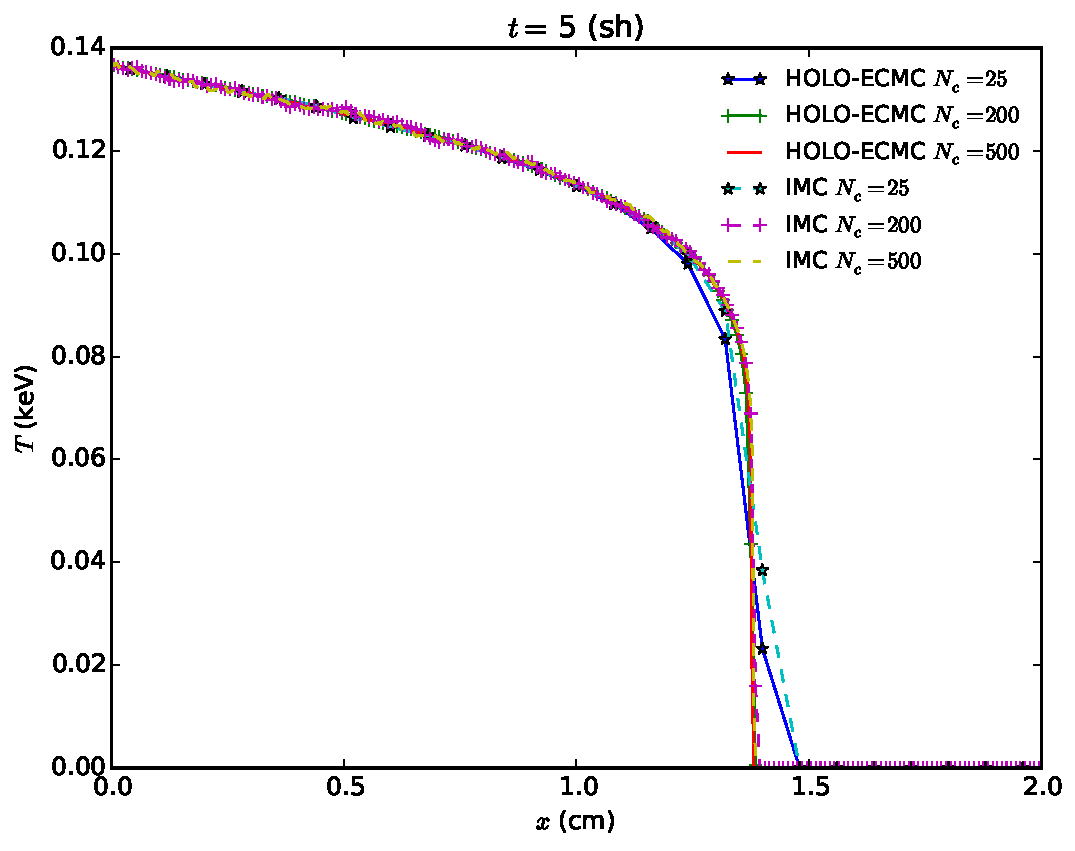
\includegraphics[width=0.99\linewidth]{marshak_mesh_conv.pdf}
    \caption{\label{marshak_mesh_conv} Convergence of IMC and HOLO-ECMC solutions.}
\end{subfigure}
\begin{subfigure}{0.7\textwidth}
  \centering
  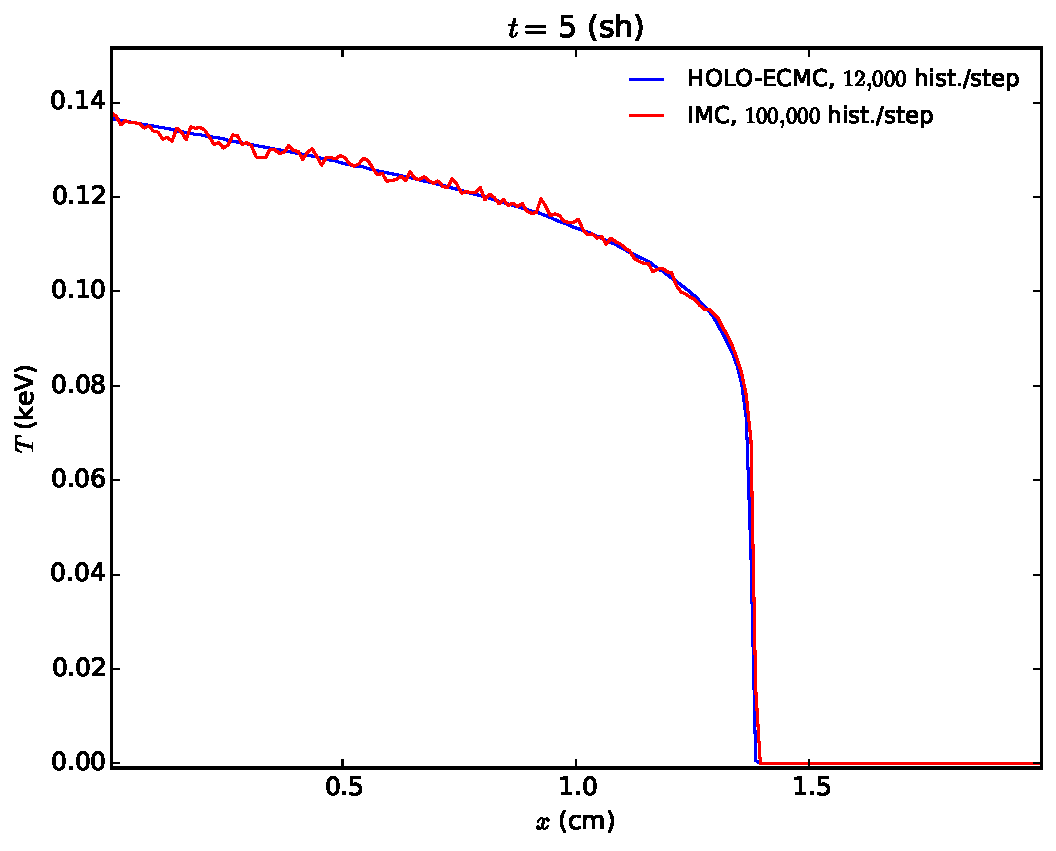
\includegraphics[width=0.99\linewidth]{marshak_200_compare.pdf}
  \caption{\label{marshak_200_compare}  Comparison of solutions for 200 spatial cells. }
\end{subfigure}
\caption{\bf Comparison of radiation temperatures for Marshak wave problem at $\mathbf{t=5}$ sh.}
\end{figure}

Fig.~\ref{marshak_mesh_conv} compares the cell-averaged radiation temperatures  for the
IMC and HOLO method with ECMC, for various number of spatial mesh cells $N_c$; we
have used HOLO-ECMC to denote our algorithm because later results will use different HO solvers.   For
all IMC calculations, $n=10^5$ histories per time step were used.  For the HOLO method, we have used
4 equal-sized cells in $\mu$ for the finite-element angular mesh used by the ECMC
solver.  The spatial grid is the same for the HO and LO solvers. For the cases
of $N_c=25$ and $N_c=200$, $4,000$ histories per batch ($n=12,000$ per time step)
were used.  For $N_c=500$, 16,000 histories per time step were used due to increased
number of space-angle cells that
need to be sampled. The IMC and HOLO solutions agree as the mesh is converged.  There is
similar agreement in the location of the wave front due to the linear shape of the emission source over a cell.  The cells
nearest the wave front required use of the lumping-equivalent discretization and
$S_2$ equivalent terms during the LO
solve, resulting in strictly positive solutions.
 
Fig.~\ref{marshak_200_compare} compares solutions
for the case of 200 cells.  For the IMC solution $10^5$ histories per time step were
simulated; for the HOLO method only $4,000$ histories per batch
(12,000 per time step) were simulated. There is significant statistical noise in the IMC solution
compared to the HOLO solution.  The HOLO solution visually demonstrates no
statistical noise.  Because the ECMC solve is only determining the change over the
time step, the statistical noise in the result is small relative to the magnitude of
$I^{n+1}$.  Also, the source sampling only places particles in cells where the residual is
large.  No particles are sampled in the equilibrium region out front of the wave. 

Table~\ref{marshak_var} compares $\ss$ and the FOM for IMC and the HOLO method, for different
numbers of histories per time step. The FOM results are normalized to the value for IMC with
$n=12,000$.  The HOLO method demonstrates less variance
for the same numbers of histories.  Where as the FOM remains relatively constant for
IMC, as $n$ is increased the FOM improves for the HOLO method.  This is a result of
each batch producing more statistically accurate estimates of the error $\epsilon$,
which results in an increased convergence rate of $\epsilon$ overall.  
\begin{table}[H]
\centering
\caption{\label{marshak_var} \textbf{Comparison of sample statistics for the Marshak Wave problem.   Simulation end time is $\mathbf{t=5}$ sh.}}
\vspace{-0.1in}
\begin{tabular}{|c|cc|cc|}\cline{2-5}
    \multicolumn{1}{c|}{}       & \multicolumn{2}{|c|}{\ss} &
    \multicolumn{2}{|c|}{\FOM} \\ \hline
hists./step   & IMC & HOLO-ECMC &  IMC & HOLO-ECMC   \\ \hline
   12,000	 & 3.40\%  & 0.28\% &  1    &  145      \\
  100,000    & 1.22\%  & 0.057\% & 0.93    &   422     \\ \hline
\end{tabular}
\end{table}



\subsection{Two Material Problem}
\label{sec:two}

This problem consists of an optically thin (left) and an optically thick (right) material region,
with temperature-independent cross sections.  The material properties are given in
Table~\ref{two_mat_props}.  Initially the radiation and material energies are in
equilibrium at a temperature of 0.05 keV.  An isotropic incident intensity of 0.500 keV
is applied at $x=0$ at $t=0$; the isotropic incident intensity on the right boundary is 0.05
keV.  The simulation is ran for 5 sh. For all HOLO simulations, we have used 8
equal-sized mesh cells in $\mu$. As for the Marshak problem, the cells nearest the wave front required use of the lumping-equivalent discretization and
$S_2$ equivalent terms during the LO solve.
\begin{table}[H]
        \caption{Material properties for two material problem\label{two_mat_props}}
\centering
        \begin{tabular}{|c|cc|}  \cline{2-3}
            \multicolumn{1}{c|}{}   & $x \in [0,0.5)$ cm & $x \in [0.5,1.0]$ cm   \\ \hline
            $\sigma_a$ (cm$^-1$)  & 0.2 & 2000 \\
            $\rho$ (g cm$^-3$) & 0.01 & 10.0 \\
            $c_v$ (jks/keV-g) & $0.1$ & $0.1$ \\ \hline
        \end{tabular}
\end{table}
Fig.~\ref{twomat_full} compares the HOLO and IMC radiation 
temperatures at the end of the simulation. The
IMC and HOLO results show good agreement
over the finer mesh.
On the coarse mesh ($N_c=20$), the LDFE representation of $T^4$ in the HOLO method predicts the location of the
wave front more accurately than the IMC method with source tilting.

Fig.~\ref{compare_ho} demonstrates the benefit of ECMC as a HO solver compared to
standard MC.  The HOLO algorithm
with the ECMC HO solver (HOLO-ECMC) results
are for running 3 batches of 10,000 histories, per time step. The solution for the HOLO method with a standard MC solver as the HO solver
(HOLO-SMC) with standard source sampling uses 10$^5$ histories per time step. The HOLO-SMC solution demonstrates significant
statistical noise.  This noise is introduced into the LO solver by bad statistics in
computing the consistency terms. Also
plotted is an S$_2$ solution obtained with consistency terms that are equivalent
to S$_2$ and no HO correction.  The S$_2$ solution results in an artificially fast
wave front, as expected, demonstrating the necessity of HO correction in this problem.

Table~\ref{twomat_var} compares the FOM and $\ss$ for IMC and the HOLO-ECMC method.  The FOM
values are normalized to the value for IMC with $n=30,000$.  The end time was reduced
to $2$ sh for these results to reduce computational times. The reduction in variance by
the HOLO method over IMC is substantial. The improvement of the FOM for the HOLO
method compared to IMC is greater than for the
Marshak wave problem.  This improvement is because the wave moves much slower in
right region of this problem, due to
the large, constant cross section.  Also, in the optically thin
region of the problem the solution quickly comes to equilibrium.  Thus, the ECMC
algorithm has to estimate a very small change in the intensity over a time step.  Additionally, difficulties in resolving
the solution at the wave front are not as severe compared to the Marshak wave
problem, where the cold cells have a much larger cross section.
\begin{figure}
    \centering
\begin{subfigure}{0.65\textwidth}
    \centering
    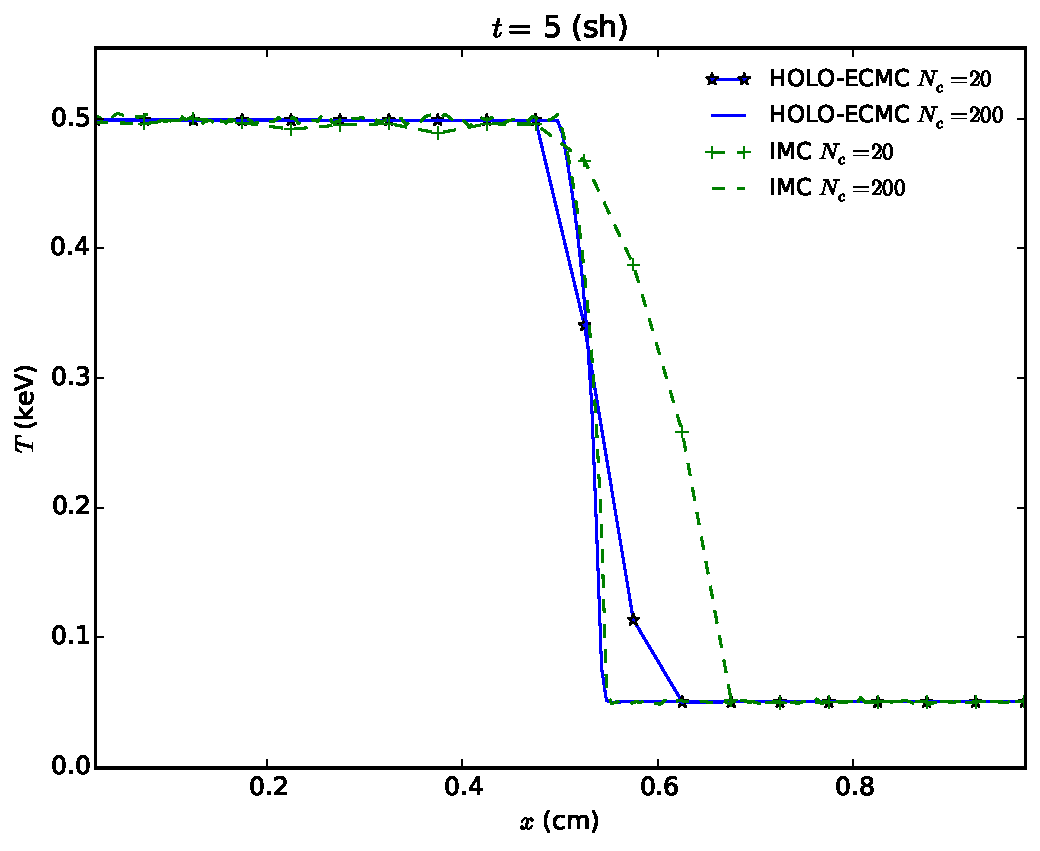
\includegraphics[width=0.99\textwidth]{two_mat_conv.pdf}
    \caption{Comparison of IMC and HOLO-ECMC.\label{twomat_full}}
\end{subfigure}    \begin{subfigure}{0.65\textwidth}
\centering
    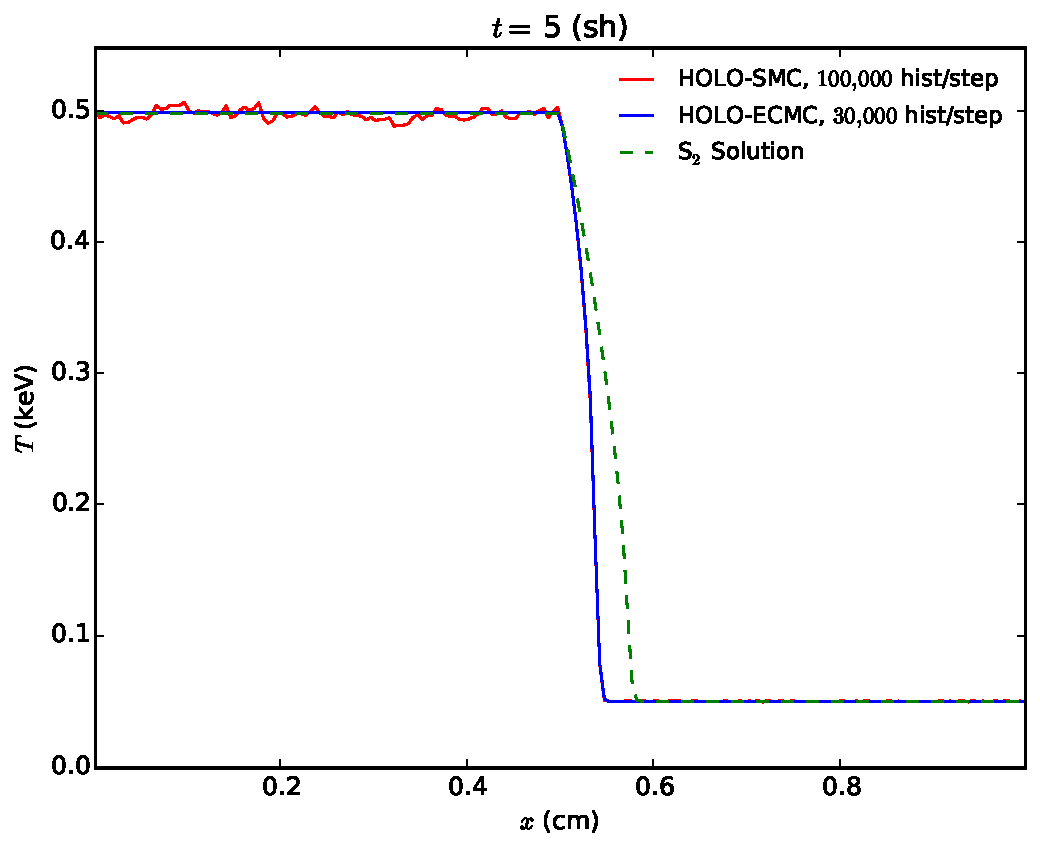
\includegraphics[width=0.99\textwidth]{two_mat_ho_compare.pdf}
    \caption{Comparison of SMC and ECMC HO solvers. \label{compare_ho}}
\end{subfigure}
    \caption{\bf Comparison of radiation temperatures for two material problem. \label{twomat}}
\end{figure}


\begin{table}[H]
\centering
\caption{\label{twomat_var} \textbf{Comparison of sample statistics for the
    two material problem for 200 $x$ cells.   Simulation end time is $\mathbf{t=2}$ sh.}}
\vspace{-0.1in}
\begin{tabular}{|c|cc|cc|}\cline{2-5}
    \multicolumn{1}{c|}{}       & \multicolumn{2}{|c|}{\ss} & \multicolumn{2}{|c|}{$s_{\max}$} \\ \hline
hists./step     & IMC & HOLO-ECMC  &  IMC & HOLO-ECMC   \\ \hline
   30,000	    & 3.63\%  & 0.01\% &  1      &   104,000      \\
  100,000       & 1.96\%  & 0.003\% & 1.03   &   360,000      \\ \hline
\end{tabular}
\end{table}

\subsection{Performance comparison of IMC and HOLO-ECMC}
\label{timing}

We have measured the total CPU time for simulations to provide a simplified measure of the
computational cost.  These results compare how computational times change the two
different problems and how the methods scale with time step size and particle histories.  Absolute comparisons in the computational cost of the two
methods cannot be made because the methods are implemented
in different code infrastructures. Additionally, the HOLO method fully resolves
non-linearities at each time step, whereas IMC is using a single linearized step with
lagged cross sections. Simulations were performed on the same processor, using a single CPU
core.  Reported times are the average of 10 runs and all results used 200 $x$ cells,
$\Delta t = 0.001$ sh, and an end time of $t=2$ sh.

Table~\ref{marshak_table} compares the average
simulation time per history performed for the Marshak wave problem.  The average time per history is computed by dividing the total simulation time by
the total number of histories performed (e.g., the time of the LO solves is included for
the HOLO method).  Results are given for different numbers of histories per time step, as
well as a case with an increased time step size.  The table also includes the number of LO
iterations performed per LO solve for the HOLO method, averaged over all time steps;
there are two LO solves per time step.  The same results are reported for the two
material problem in Table~\ref{twomat_table}.

The HOLO method does not scale with the number of
histories due to the fixed cost of the LO solver.  The cost of the LO solver is more
significant at the lower history counts compared to the case of $10^5$
histories, for both problems. 
There is a slight increase in the number of
newton iterations as the time step is increased, but the average cost per history is
not significantly increased.   Similar to the results
in~\cite{park}, as the time step size is increased to to 0.005 sh, the IMC method
increases in cost per time step, particularly for the two material problem. Because
the cross sections in the the two material problem do not have a $T^{-3}$
behavior,the cost of the effective scattering cross section in IMC is more apparent,
resulting in longer simulation times. 
\begin{table}[H]
\centering
\caption{\label{marshak_table} \textbf{Comparison of average CPU times per history
    and LO iteration counts for the Marshak Wave problem. }}
\vspace{-0.1in}
	\begin{tabular}{|cc|c|cc|}\hline
hists./step & $\Delta t (sh)$ & IMC ($\mu$s/hist.) & HOLO-ECMC ($\mu$s/hist) & Iters./LO solve \\ \hline
10$^5$                    &   0.001	& 10  &  5.3   & 3.8               \\
$1.2\times10^4 $          &   0.001	& 9.7 &	 8.1   & 4.1               \\
$1.2\times10^4$           &   0.005	& 19  &  9.4   & 6.2                \\ \hline
\end{tabular}
\end{table}

\begin{table}[htb!]
\centering
\caption{\label{twomat_table} \textbf{Average CPU times per history and LO iteration
counst required for the two material problem.}}
	\begin{tabular}{|cc|c|cc|} \hline
hists./step & $\Delta t (sh)$ & IMC ($\mu$s/hist.) & HOLO-ECMC ($\mu$s/hist)  &  Iters./LO Solve\\ \hline
10$^5$            &   0.001	& 17  &	3.5   & 4.9 \\
$3\times10^4 $   &    0.001	& 18  &	6.9   &    5.0 \\
$3\times10^4$     &   0.005	& 59  & 7.4   &    7.6 \\ \hline
\end{tabular}
\end{table}

\subsection{Comparison of different HO Solvers}
\label{ho_solvers}

In this section we compare the results of our HOLO algorithm with different HO
solvers for the test problems in Section~\ref{sec:marsh} and~\ref{sec:two}.  We compare standard MC (SMC) as a HO solver to the HOLO algorithm with ECMC using
both three batches and a single batch, per time step.  The use of a single batch is
similar to the approach in~\cite{rmc}.  Results are tabulated for 200 $x$ cells, using the same total
number of histories per time step, divided evenly among the batches.

Tables~\ref{homarshak_var} and~\ref{hotwomat_var} compare the results for the Marshak
wave and two material problems. The number of batches for each ECMC case is indicated
in parenthesis.  The FOM values are normalized to the reference IMC result for the
corresponding problem.  For HOLO-SMC there is
minimal reduction in variance compared to IMC in the Marshak wave problem, and the two
material problem actually demonstrates worse variance.  Sufficient histories are not
performed to accurately estimate consistency terms throughout the problem.  For ECMC,
a single batch produces less variance than the case of three equal batches.  This
indicates that if the solution cannot be resolved with the trial space (i.e., the
intensity is driven negative), a single large batch may be more accurate. It is noted
that these results only account for statistical variance, and do not account for
accuracy, which will depend on the the estimates of $\epsilon$ computed each iteration.   

\begin{table}[H]
\centering
\caption{\label{homarshak_var} \textbf{Comparison of sample statistics for the Marshak Wave problem.  Number of ECMC batches is
indicated in parenthesis.}}
\vspace{-0.1in}
\begin{tabular}{|c|ccc|ccc|}\cline{2-7}
    \multicolumn{1}{c|}{}       & \multicolumn{3}{|c|}{\ss} &     \multicolumn{3}{|c|}{\FOM} \\ \hline
hists./step   & SMC & ECMC (1) & ECMC (3)  & SMC & ECMC (1) & ECMC (3)   \\ \hline
   12,000	   & 2.77\%  & 0.10\% &  0.28\% &   1.50    & 1280  & 145     \\
  100,000      & 0.98\%  & 0.03\% &  0.06\% &   1.43    & 1270  & 422     \\ \hline
\end{tabular}
\end{table}


\begin{table}[H]
\centering
\caption{\label{hotwomat_var} \textbf{Comparison of sample standard deviations for the
    two material problem. Number of ECMC batches is indicated in parenthesis.}}
\vspace{-0.1in}
\begin{tabular}{|c|ccc|ccc|}\cline{2-7}
    \multicolumn{1}{c|}{}       & \multicolumn{3}{|c|}{\ss} &
    \multicolumn{3}{|c|}{\FOM} \\ \hline
hists./step   & SMC & ECMC (1) & ECMC (3)  & SMC & ECMC (1) & ECMC
(3)   \\ \hline
   30,000	  & 5.35\%   & 0.002953\% & 0.011\%  & 0.46     & 1.51$\times10^6$   & $1.04\times10^4$          \\
  100,000     & 2.85\%   & 0.001474\% & 0.0033\% & 0.49     & 1.80$\times10^6$   & $3.59\times10^4$          \\ \hline
\end{tabular}
\end{table}

\subsection{Pre-heated Marshak wave problem and adaptive mesh refinement}

Finally, to demonstrate the potential of ECMC with adaptive space-angle mesh refinement, we perform
results for a modified Marshak wave problem. The problem is modified so that the LDFE
trial space can accurately represent the solution (i.e., the intensity is strictly
positive).  Mesh refinement is of minimal use in the previous problems due to most of
the error existing at the wave fronts, caused by the large cross sections.   The modified problem has the same material
properties and left boundary source as the Marshak wave problem in
Section~\ref{sec:marsh}.  However, the initial equilibrium
temperature and right boundary condition are raised to $0.03$ keV.   The higher initial temperature reduces the
initial cross section and increases the strength of the emission source within cells.  
The LDFE mesh can now sufficiently resolve the solution and lumping is
not required by the LO solution.  The simulation end time is 0.5 sh with a constant
time step of $\Dt=0.001$ sh.  

Fig.~\ref{hot_plot} compares the result from HOLO-ECMC with three batches and IMC.
It was found that 100 $x$ cells was sufficient to resolve the solution spatially. There is slightly more noise in IMC past the wave front due to the increased emission
source.  Additionally, the opacity is thin enough that some photon energy is able to
reach the right boundary, in front of the wave front. 

Table~\ref{preheat_var} compares the variances for this problem for the various HO
solvers. The FOM values are normalized to the case of HOLO-SMC with 12,000
histories per time step. The final row of the table is for an ECMC simulation with adaptive mesh
refinement (AMR).  The strategy for refinement is described in
Appendix~\ref{app:refinement}.  The adaptive
mesh refinement case used a total of nine batches, with a refinement occurring at the end
of the third and sixth batches, for every time step. The initial number of histories was adjusted so that
the average number of histories per time step is near 100,000; on average 99,881
histories per time step were used.  All ECMC meshes used 4 equally-spaced $\mu$ cells
initially. 
   The improvement in variance by ECMC compared to SMC is not as significant
as for the other problems.  This is a
result of the reduced opacity leading to intensity changing throughout the spatial
and angular domains.  The
FOM is highest for the case of ECMC with adaptive refinement. When the solution can
be resolved, the adaptive algorithm allows for a higher convergence rate of
statistical variance.  It is noted that the consistency terms and LO solution are still computed over
the fixed, coarser mesh.  However, in general, the refined mesh can produce higher accuracy in consistency terms that is
not being measured by the FOM.
\begin{figure}[htb]
  \centering
    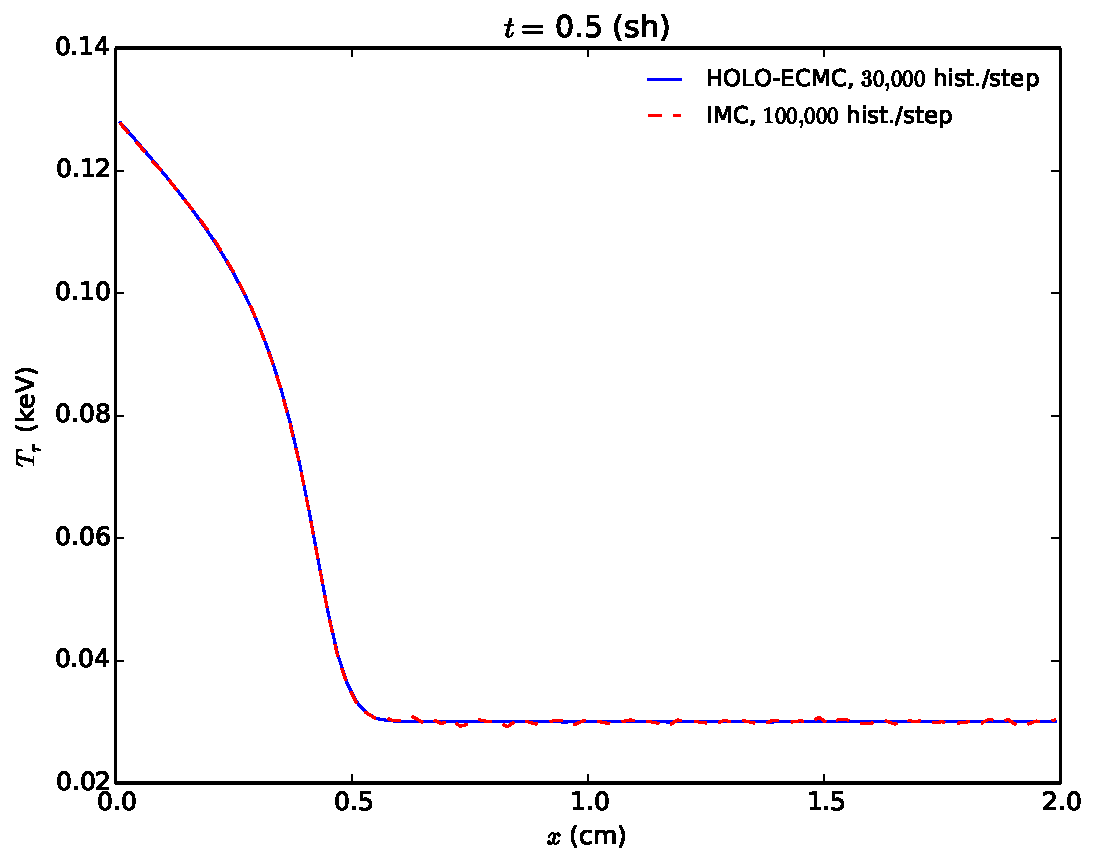
\includegraphics[width=0.65\textwidth]{heated_marshak.pdf}
    \caption{\label{hot_plot}\bf Comparison of radiation temperatures for the pre-heated Marshak wave problem for 100
    $x$ cells at $\mathbf{t=0.5}$ sh.}
\end{figure}


\begin{table}[H]
\centering
\caption{\label{preheat_var} \textbf{Comparison of sample statistics for the 
    pre-heated marshak wave problem for 100 $x$ cells. Number of ECMC batches is
indicated in parenthesis.}}
\vspace{-0.1in}
\begin{tabular}{|c|ccc|ccc|}\cline{2-7}
    \multicolumn{1}{c|}{}       & \multicolumn{3}{|c|}{\ss} &
    \multicolumn{3}{|c|}{\FOM} \\ \hline
hists./step   & SMC & ECMC (1) & ECMC (3)  & SMC & ECMC (1) & ECMC (3)   \\ \hline
   12,000	  & 0.86\%   & 0.13\% & 0.24\% & 1      & 41  & 13      \\
  100,000     & 0.16\%   & 0.042\% & 0.08\% & 3.32   & 52  & 15       \\
  99,881 (AMR) & --  & --  & 0.038\% & -- & -- &   61               \\ \hline
\end{tabular}
\end{table}


\section{CONCLUSIONS}

We have been able to produce solutions for Marshak wave test problems using
a new HOLO method that are in agreement with IMC.  Unlike IMC, our method requires no effective scattering
events to be included in the MC simulation, which limits the run time of particle
tracking, while adding the cost of a LO newton solver. Average LO iteration counts
did not significantly increase as the time step size was increased. The LDFE spatial representation
mitigates issues with teleportation error, producing results with spatial accuracy
comparable to IMC with source tilting.  The ECMC approach, with initial guesses based on the
previous radiation intensity, results in efficient reduction of statistical error and
allows for particles to be distributed to largely varying regions of the problem.
The LO solver resolves the non-linearities in the equations resulting in a fully
implicit time discretization
The LO solver
can accurately and efficiently resolve the solution in diffusive regions, while the HO
transport solver provides the accuracy of a full transport treatment where necessary. 

The primary difficulty to overcome in the ECMC algorithm is when the solution cannot
be accurately represented by the trial space, e.g., in optically thick cells where
the solution is driven negative.   We are currently developing an approach to allow
the ECMC iterations to continue converging globally when there are such regions
present.  It is necessary to ensure the
 closure in the LO system is consistent with the HO
representation for the solution in such regions.  The ability to represent the solution accurately in
rapidly varying regions of the problem will be key for generalization of this method
to higher dimensions.  A formulization of the ECMC method
that allows for time-continuous MC transport (similar to IMC) is also currently being
investigated.  This may reduce some of the loss of accuracy in optically thin regions
due to the time discretization of the transport equation in the HO solver.
However, greater time accuracy is not of primary concern as this method is intended
for use in problems dominated by large absorption opacities, where the
absorption-reemission physics make the LO acceleration is critical.  

Future work will also explore the accuracy of the HOLO method, in particular,
analyzing the optimal number of batches and the benefit of adaptive refinement.  This will likely
require the use of manufactured solutions.  The sensitivity of the method to mesh sizes and time step sizes will be
investigated more thoroughly.  
Ultimately, we plan to extend this method to multiple spatial dimensions for the 
case of multigroup TRT equations.  For TRT problems, it is important that
the LO spatial discretization satisfies the equilibirium diffusion limit.  To extend
to higher dimensions, our LDFE representation may require the use of a higher-degree
spatial representation for the LO system to achieve the diffusion
limit. Further asymptotic
analysis on the method will be applied before implementation. It may be necessary to use a different LO system (e.g., the non-linear diffusion
acceleration approach in~\cite{rmc}), if the S$_2$-like equations become too
inefficient or difficult to implement in higher dimensions.  Alternatively, a
variable Eddington Tensor approach may provide more stability in rapidly variable
regions of the problem while still allowing for a consistent, LDFE solution that is efficiently solvable.

\section*{ACKNOWLEDGEMENTS}

This research was supported with funding received from the DOE Office of Nuclear
Energy's Nuclear Energy University Programs, the DOE National
Nuclear Security Administration, under Award Number(s) DE-NA0002376, and under Los Alamos National Security,
LLC, for the National Nuclear Security Administration of the U.S. Department of
Energy under contract DE-AC52-06NA25396. 

\pagebreak

% This includes all references from the BibTeX file in the bibliography
\nocite{*}

\begin{spacing}{1}
  \bibliographystyle{plain}
  \bibliography{references}
\end{spacing}

\end{document}
